\chapter{Game Tags in Audio Visual Collections}\label{chap:kcap}
\begin{quotation}
\noindent
In this chapter we study the characteristics of the user tags collected with the video labelling game \textit{Waisda?}. We address two aspects related to the user tags. First, we investigate to what extent does the terminology employed by the users when tagging videos differ from the terminology used by the professional cataloguers. Second, we examine which facets (\textit{who}, \textit{what}, \textit{where}, and \textit{when}) of the videos tagged by the users are typically described by the user tags and what is the level of specificness (\textit{abstract}, \textit{general}, and \textit{specific}) of the said tags. 
The findings in this chapter outline some of the strengths but also the limitations of the user tags. Our analysis shows that there is a terminological gap between the players of \textit{Waisda?} and the professionals. This makes the user tags a valuable asset as they are \textit{from the users and for the users} and can improve the access to the videos in the case when the ones accessing are the users themselves. Furthermore,  we find that user tags predominately describe instances (objects) in the video and rarely scenes. 
This fact hints that user tags could be useful for instance search and not so useful for topical search. These matters are addressed in the following chapters.

This chapter was published as ``On the Role of User-generated Metadata in Audio Visual Collections" in the Proceedings of the International Conference on Knowledge Capture 2011 \cite{kcap}. It was co-authored with Michiel Hildebrand, Jacco van Ossenbruggen, Lora Aroyo, and Guus Schreiber. 
\end{quotation}

\section{Introduction}

Crowdsourcing has gained attention as a method to collect large numbers of
metadata descriptions for media
objects~\cite{MATW2007:Chan,MATW2009:Leason,FlickrCommons}. Based on the idea
coined by Luis von Ahn~\cite{gwap}, a specific type of crowdsourcing has
become known as Games With A Purpose (GWAP). Inspired by this idea, the
Netherlands Institute for Sound and Vision deployed the video labeling game,
\emph{Waisda?}. Unique for this initiative is that the institute
aims~\cite{johanwebsci} to integrate the game into their workflow to
complement professional cataloguing and content based retrieval
techniques~\cite{ISR2009:hollink}. More specific, with \emph{Waisda?} they aim
to collect metadata in a user vocabulary that describes the content within the
video.

We investigate to what extent the aims of Sound and Vision are fulfilled by
analyzing the 420,000 user tags collected during the first pilot with
\emph{Waisda?}. To determine the vocabulary used by the crowd, we compare the
tags with existing controlled vocabularies. We compare the tags with the
professional metadata by matching them to terms of the institutes' in-house
thesaurus. Additionally, by matching the tags to the terms of a Dutch
linguistic database, we conclude that a large part of the tags are Dutch words
not used by professionals. To determine the type of content that the tags
describe we first compare them with the subtitles. Finally, we manually
classify the tags from a small number of videos. Using an existing
classification model, we show the relation between the content in the video
that is described and the type of tags that are used for these descriptions.

The rest of the paper is structured as follows. Section \ref{sec:related_work}
discusses related work. Section \ref{kcap:sec:approach} presents the approach we
take in tackling the goals we set forth. Section \ref{kcap:sec:materials} describes
the materials we used in our study. Section \ref{sec:experiments} reports on
the various experiments we performed on the user tags. Finally, section
\ref{sec:discussion} draws conclusions and points to some further directions
for research.

\newpage

\section{Related work}
\label{sec:related_work}

\subsection{Games with a purpose}

Games with a purpose (or GWAPs) are computer games, in which people, as a side
effect of playing, perform tasks computers are unable to perform \cite{gwap}.
The first example of a GWAP was the ESP game \cite{CHI2004:vonAhn}, designed
by Luis von Ahn, which harnesses human abilities to label images. The game
randomly pairs up two players with the task to describe images. When both
players provide the same label for an image, they score points and proceed to
the next image. The labels entered by both users are associated to the image
as metadata. In other words, the consensus among users provides a method to
ensure the quality and consistency of the labels. Evaluation shows that these
labels can be used to retrieve images with high precision and are almost all
considered as good descriptions in a manual assessment.

The idea to collect metadata through games with a purpose has been applied to
video footage in, for example, the Yahoo! video tag game
\cite{WWW08_vanZwol_etal},
VideoTag\footnote{\url{http://www.videotag.co.uk/}},
PopVideo\footnote{\url{http://www.gwap.com/gwap/gamesPreview/popvideo/}} and
\emph{Waisda?}. The gameplay of these video labeling games differs from the
ESP game in two ways: (i) multiple users can participate in a single game, and
(ii) the users score points when the same tag is entered in a specific time
interval. The underlying assumption is that tags are probably valid ---
trustworthily describe the video fragments --- if they are entered
independently by at least two players within a given time-frame. From here on
we shall refer to tags that are mutually agreed on as \textit{verified} tags.

Compared to the other video labeling games, \emph{Waisda?} is unique in the
sense that it is initiated by an audiovisual institute with the purpose to
improve access to their collection~\cite{johanwebsci}. With \emph{Waisda?} the
Netherlands Institute for Sound and Vision aims to collect metadata in a user
vocabulary, as it is suggested that such metadata can help bridge the gap
between the search queries and the indexing vocabulary~\cite{Jorgensen2007}.
In addition, it is expected that the resulting time-related metadata of the
content within the video can improve support for finding fragments within
entire broadcasts~\cite{bouke}. We investigate to what extent the tags
collected in \emph{Waisda?} provide a user vocabulary and analyze what type of
content within the video they describe.

\subsection{Evaluation of end-user tags}

The steve.museum research \cite{MATW2009:Leason} was one of first attempts to explore
the role of user-generated metadata. In this collaboration of several art
museums a collection of artworks was made available to the general public who
were asked to tag them. Among other things, the project studied the
relationship of the resulting folksonomy to professionally created museum
documentation. The results showed that users tag the artworks of art from a
perspective different than that of museum documentation: around 86\% of tags
were not found in museum documentation. We perform a similar study on the
collection of \emph{Waisda?} tags by comparing them to in-house thesaurus.

Museum staff also assessed the tags from the steve.museum project on
usefulness when used to search for artworks. From the total number of tags,
88.2\% were found to be useful. Following the methodology of steve-museum,
Netherlands Institute for Sound and Vision also asked a senior cataloguer to
judged a sample of \emph{Waisda?} tags on their usefulness when searching for videos
\cite{waisda}. The sample consisted of the 20 most frequent and the 20 least
frequent tags from two television programs. The cataloguer found the majority
of the tags to be useful. She also noted that there seems to exist a
difference between professional descriptions and end-user tags. While
professionals describe the topical subject of the program, the players in
\emph{Waisda?} generally tag things that can be directly seen or heard in the
video. One of the aims of this paper is to investigate the characteristics of
the tags and what they describe in the video more methodically, and on a
larger scale.

There is substantial body of research work that investigates user tags and
folksomies. For example, in~\cite{citeulike:468899, citeulike:1421739} the
overall quality of end-user tags is examined and the main strengths
(flexibility, simplicity, user perspective, etc.) and potential weaknesses
(typos, morphological variation of words, no synonym and no homonym control,
etc.) are pin-pointed. Gruber~\cite{gruber_2007} identifies the roles of
folksonomies and formal vocabularies and presents use-cases where both can
naturally co-exist and cooperate. While many aspects of user tags are well
covered in research, little or no attention is paid to the link between tags
and the resources they are referring to. In this study we investigate which
aspects of the resources (in our case videos) are covered by user tags.

\subsection{Classification of user descriptions} 

Various schemes have been developed for classification of user descriptions
for visual resources. One of the first is the Panofsky-Shatford model
\cite{Panofsky, Shatford} which focuses on the conceptual descriptions. Jaimes
and Chang \cite{Jaimes00aconceptual} developed a classification framework for
visual resources (including video) that besides conceptual descriptions also
considers perceptual (low-level features) and non-visual descriptions. Hollink
at al. \cite{laurapaper} combined the previous two schemes and developed a
classification framework for user descriptions. As we exploit this framework
to classify end-user tags, we explain it in more detail in the following
section.

\subsubsection{Tag classification framework}\label{tag_class_framework}

The framework distinguishes three top-levels: nonvisual level, perceptual
level, and conceptual level. Descriptions at nonvisual level are meant to
describe the context of the video but not its content. This is in contrast
with descriptions at perceptual and conceptual level which are referring
solely to the content of the video. Nonvisual level includes the following
classes: \textit{creator}, \textit{title}, \textit{date}, \textit{location},
\textit{carrier type}, etc.

Descriptions at perceptual level are derived from low-level audio and visual
features of the video. In principle, no domain and no worldly knowledge is
required to create descriptions at this level. Perceptual level classes are
divided into classes of descriptions that refer to visual features such as
\textit{color}, \textit{shape}, and \textit{texture} and classes of
descriptions that refer to audio features like \textit{volume},
\textit{pitch}, and \textit{amplitude}.

Descriptions at conceptual level describe the semantic content of the video.
To classify tags at this level the Panofsky-Shatford model is used. This model
divides conceptual descriptions into three levels: \textit{general} (generic
things in the video), \textit{specific} (specific things), and
\textit{abstract} (symbolic things). Each of the levels is further broken down
into four facets: \textit{who}, \textit{what}, \textit{where}, and
\textit{when} producing the Panofsky-Shatford 3x4 matrix. 

In addition, descriptions may be about \textit{visual objects} or may refer to
the entire scene. We take the approach of \cite{Jaimes00aconceptual} and
define visual objects as entities that can be seen, sometimes differing from
the traditional definition of object. Objects like the sky or the ocean would
perhaps not be considered objects under the traditional definition, but
correspond to our visual objects (as well as the traditional objects like car,
house, etc.). Examples of scene descriptions include city, landscape, indoor,
outdoor, still life, portrait, etc.


\section{Approach}\label{kcap:sec:approach}

We divided our study of the \emph{Waisda?} data in two parts. In the first
part we focus on the user tags, investigating the vocabulary that users employ
when describing videos. We analyse the relationship to the vocabularies used
by professional cataloguers and general web users. In the second part we focus
on what the users describe. We analyse which aspects of the video are
described and what type of tags are used for this.

With respect to the first part, we perform the following experiments. First, in order to estimate the lower bound of the fraction of user tags that are proper words, we examine the overlap between them and a general lexicon of the Dutch language. Furthermore, to determine if
users and professionals use different vocabularies when describing videos, we
investigate the overlap between all user tags and a typical domain thesaurus
used by professionals in the cataloging process. A significant part of the
non-verified tags --- not entered by at least two different users --- are not
found in the either of the vocabularies we consider. To understand if these
tags are just gibberish or actually have meaning we perform additional
experiment using the Google\footnote{http://www.google.com} search engine as
semantic filter: we deem a tag as meaningful only if the number of pages
returned by Google is positive. The procedure is motivated by the intuition
that if a person has used a word or a phrase on the Web then it probably has
some meaning. Subsequently, to shed more light on this potentially useful
class of tags we select samples from both the tags found and not found by
Google for further inspection.

With respect to the second part, we take a combined approach. First, we
investigate what do users tend to describe more: things \textit{heard} or
things \textit{seen} on screen. To this end we perform a study on the overlap
between the user tags and the audio signal --- subtitles for hearing impaired
persons --- for a sample of episodes. To get a more comprehensive
understanding of the types of tags users usually add, we perform a qualitative
study of a sample of user tags obtained through the \emph{Waisda?} video
tagging game. In the course of the study each tag is manually analyzed in the
light of the video content it describes and categorized in terms of the
classification framework described in section \ref{tag_class_framework}.

\section{Materials}\label{kcap:sec:materials}
In this section we describe the materials and resources used in the study.

\subsection{Waisda? data snapshot}\label{waisda_ds}

Subject of our analysis is the data collected in the first pilot project with
\emph{Waisda?}, a period starting from the launch date in May 2009 until 6th
of January 2010. During this period, the game amassed over 46,000 unique tags
ascribed to approximately 600 videos by roughly 2,000 different
players\footnote{Throughout this text we use the terms \textit{player} and
\textit{user} interchangeably }. The number of distinct tag entries exceeded
420,000. The database of the game contains information about players, games,
videos, and tag entries. Each tag entry is represented by an instance of a
ternary relation that relates the player that entered the tag, the video the
tag was attached to, and the tag itself. Additionally, a tag entry is
associated with the point in time --- relative to the beginning of the video
--- when the tag was entered. It also includes a score computed taking into
consideration agreement with other tag entries in the temporal neighborhood.
Since almost all players originate from the Netherlands and all videos
subjected to tagging are in Dutch, the language of the vast majority of tags
-- nearly 100\% --- is Dutch.

\subsection{Domain and lexical vocabularies}\label{vocs}
For this study we used two vocabularies: GTAA and Cornetto. While the former is a domain vocabulary, the latter is a general lexical source that covers common lexical terms.

GTAA (Dutch acronym for Common Thesaurus Audiovisual Archives) is the thesaurus used by professional cataloguers in the Sound and Vision documentation process. It contains approximately 160,000 terms divided in six disjoint facets: subjects or keywords ($\approx$ 3,800 terms), locations ($\approx$ 17,000 terms), person names ($\approx$ 97,000 terms), organization-group-other names ($\approx$ 27,000 terms), maker names ($\approx$ 18,000 terms) and genres (113 terms). GTAA terms are interlinked with each other and documented using four properties: Broader Term, Narrower Term, Related Term and Scope note. While all GTAA terms may have related terms and scope notes, only terms from subject and genres facet are allowed to have narrower and broader terms. Complementary to the narrower/broader term hierarchy, terms from the subject facet are classified by theme in 88 subcategories which are organized into 16 top-level categories.

Cornetto is a lexical semantic database of Dutch that contains 40K entries, including the most generic and central part of the language. It is build by combining Dutch Wordnet (DWN) with Referentie Bestand Nederlands (RBN) which features FrameNet-like information for Dutch \cite{Vossen08}. Cornetto organizes nouns, verbs, adjectives and adverbs into synonym sets called \textit{synsets}. A synset is a set of words with the same part of speech that can be interchanged in a certain context. Synsets are related to each other by semantic relations --- like hyperonomy, hyponomy, meronomy etc. --- which may be used across part of speech. Although Cornetto contains 59 different kinds semantic relations, hyperonymy and hyponomy are by far the most frequent ones, accounting for almost 92\% of all semantic relation instances.

\subsection{Videos}\label{videos}

For the manual classification the number of programs in the \emph{Waisda?} is
too large to include all of them. In addition, subtitles are not available for
all videos. Therefore, for the manual classification and comparison with the
subtitles we opted for select a subset. We selected five episodes: the two
best-tagged videos, one averagely tagged video and two low-tagged videos. The
two best-tagged videos are episodes from a popular Dutch reality show,
\textit{Farmer seeks Wife}\footnote{http://www.bzv.kro.nl/}, categorized as
amusement. The averagely tagged video is an episode from the
\textit{Traceless}\footnote{http://spoorloos.kro.nl/} series, classified as
amusement and informative program. The two low-tagged videos are episodes from
\textit{The Walk}\footnote{http://dewandeling.kro.nl/} and
\textit{Reporter}\footnote{http://reporter.kro.nl/} series, categorized as
religious and informative, respectively. Table \ref{table:videos} summarizes
the most pertinent information about the episodes. Prior research
\cite{waisda} suggested that the program genre might in fact influence the
types of tags users add. To account for this phenomenon, we made sure that
videos and fragments of all genres are present in our sample.

\begin{table}[tb]
\centering
\begin{footnotesize}
\begin{tabular*}{\columnwidth}{@{\extracolsep{\fill}}lrrr}
\toprule
\textbf{Episode} \T \B & \textbf{All tags} & \textbf{Verified}&\textbf{Category} \\  
\midrule
Farmer seeks wife 1\B \T &25,965  & 5,837&\textit{Amusement}\\
Farmer seeks wife 2\B &22,792  &6,153  & \textit{Amusement}\\
Traceless\B& 1,007 &274& \textit{Amusement,}\\
&&& \textit{Informative}\\
%\hline
Reporter\B&403& 73&\textit{Informative}\\
%episode &&&\\
%\hline
The Walk \B &257& 45&\textit{Religious}\\
%episode&&&\\
\bottomrule
\end{tabular*}
\end{footnotesize}
\caption{Sample of waisda? episodes used in the experiments.}
\label{table:videos}
\end{table}

\subsection{Subtitles}\label{subtitles}

For the comparison of the tags with the audio signal we make use of the
subtitle files associated with the television programs. Subtitles are textual
versions of the dialog in films and television programs, usually displayed at
the bottom of the screen\footnote{Timed Text Working Group,\\ http://www.w3.org/AudioVideo/TT/}. Each dialog excerpt is accompanied with
time-points --- relative to the beginning of the video --- when the dialog
excerpt appears on and disappears from the screen. The subtitles files we use
were obtained from KRO broadcasting and are specified in the SubRip text file
format\footnote{http://en.wikipedia.org/wiki/SubRip\#SubRip\_text\_file\_\\format}.

\section{Experiments}\label{sec:experiments}

In this section we present the results from the three experiments: matching
tags to vocabularies, matching tags to subtitles and manual classification of
the tags.

\subsection{Matching tags to vocabularies}
\label{tags-in-vocabularies}

In this experiment we matched all \emph{waisda?} tags to two vocabularies: the
general lexicon of Dutch language Cornetto and the domain thesaurus GTAA. In
mapping the tags to concepts we take the following approach. We deem a tag and
GTAA term to be a positive match only if they are the same string (ignoring
case). A tag and Cornetto synset are considered a positive match only if at
least one of the words associated with the synset is equal (in
case-insensitive manner) with the tag.

\begin{table}[tb]
\begin{footnotesize}
\centering
\begin{tabular*}{\columnwidth}{@{\extracolsep{\fill}}lrlrl}
\toprule
\T \B & \multicolumn{2}{c}{\textbf{All tags}} & \multicolumn{2}{c}{\textbf{Verified}} \\
\midrule
 Total \T \B & 46,792 && 12,963&\\
 In GTAA \B & 3,850 & (8\%) & 1,825 & (14\%)\\
 In Cornetto \B & 10,939 & (23\%) & 5,669 & (44\%)\\
\bottomrule
\end{tabular*}
\caption{Overlap of \emph{Waisda?} tags with GTAA thesaurus and Dutch linguistic database, Cornetto.}
\label{tab:overlap}
\end{footnotesize}
\end{table}

The results of the mapping of \emph{Waisda?} tags against Cornetto and GTAA
are presented in table \ref{tab:overlap}. We observe that only a small part of
the unique tags are found in GTAA (8\%). A larger number of the tags are found
in Cornetto (23\%). This difference between the overlap with GTAA and Cornetto
is larger for the verified tags. Almost 44\% of the verified tags is found in
Cornetto, whereas only 14\% is found in GTAA. In other words, at least 30\% of the
verified tags are proper Dutch words but would not be used by a professional
cataloguer\footnote{GTAA contains all terms used to annotate videos in Sound
and Vision}. In addition, we observe that the verified tags are more often
valid Dutch words than the non-verified ones.

\begin{table}[tb]
\centering
\begin{footnotesize}
\begin{tabular*}{\columnwidth}{@{\extracolsep{\fill}}lrr}
\toprule
\multirow{7}{*}{\textbf{GTAA}} & \textbf{Facet}\B \T & \textbf{Tags} \\
  \cline{2-3}
 & Subject \T \B & 1199\\
 & Location \B &  613 \\
 & Genre \B & 52\\
 & Person \B & 118\\
 & Maker \B & 4\\
 & Name \B & 673\\
\hline
\multirow{5}{*}{\textbf{Cornetto}} & \textbf{Types} \B \T & \textbf{Tags} \\
\cline{2-3}
 & Noun \T \B &  7222 \\
 & Verb \B & 2090 \\
 & Adjective \B & 1693\\
 & Adverb \B & 171\\
\bottomrule
\end{tabular*}
\end{footnotesize}
\caption{Waisda? tags distribution over GTAA facets and Cornetto synset types.}
\label{tag_dist_over_Cornetto_GTAA}
\end{table}

Using the overlap with the vocabularies we can also provide a first
classification of the tags. Using the different facets in GTAA we can
distinguish different types of tags, such as subject terms, locations persons
and organization names. In WordNet we can distinguish the tags matching with
different types of words, such as noun and verb. Table
\ref{tag_dist_over_Cornetto_GTAA} shows the distribution of user tags over the
GTAA facets and Cornetto synsets. We observe that most tags are matched with
subject terms from GTAA, but also a large number of tags could be matched to
locations and names. The overlap with Cornetto shows that most tags are
matched to nouns. Surprisingly, there is also a substantial number of tags
matched with adjectives. In fact, one of the most frequently occurring tags is
the adjective, nice.

\begin{figure}[t!]
\centering
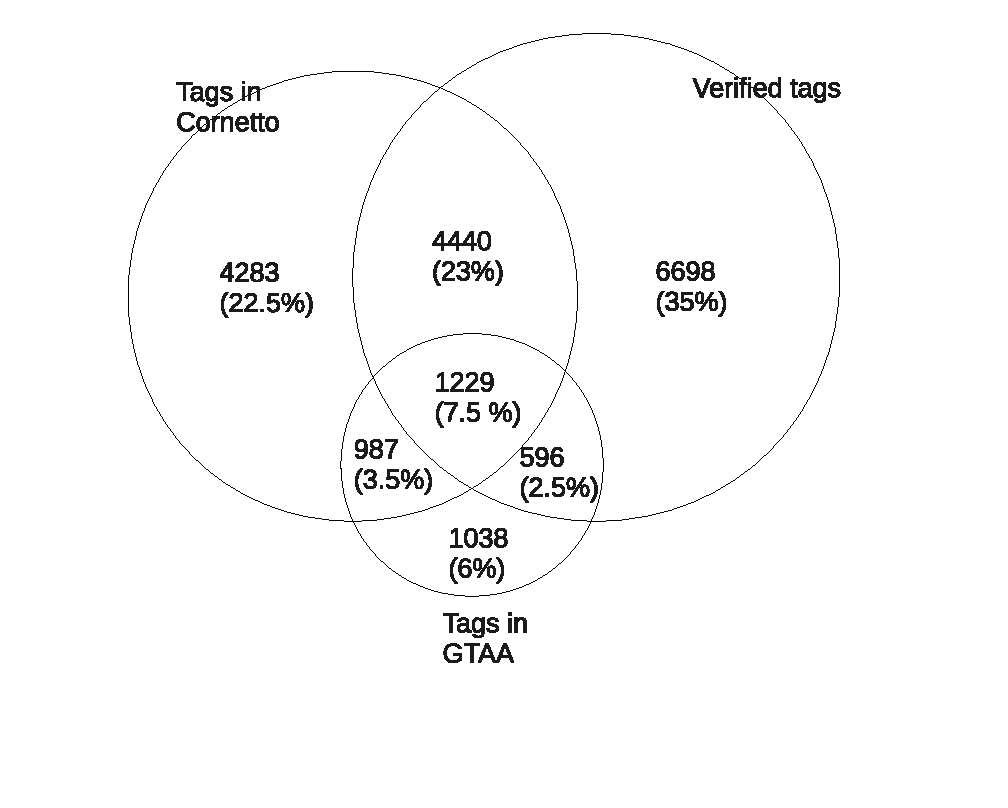
\includegraphics[width=\columnwidth, trim=0 50 0 0, clip=true]{kcap:venn-diagram.eps} 
\caption{Overlap among verified Waisda? tags,  tags in Cornetto, and tags in GTAA. %All numbers are also given as percent (fraction) of the total number of unique tags, 46,792.
}
\label{venndiagram}
\end{figure}

From the total number of tags in total 41\% are either verified or found in
one of the vocabularies. Figure \ref{venndiagram} provides a detailed view of
these tags, showing the overlap between the different sets. We observe that
35\% of the verified tags are not found in either GTAA or Cornetto. Further
investigation revealed that some of these tags do correspond to terms from the
vocabularies, but were not found by the matching algorithm. We also observe
that 32\% (the sum of 22.5\%, 3.5\% and 6\%) of the tags are found in the
vocabularies, but are not verified.

The majority of the tags, approximately 59\%, are neither found in Cornetto
and GTAA nor they are verified. Further analyses revealed that almost half of
these tags are comprised of more that one word. While this could to some
extent explain why they were not found in Cornetto and GTAA (these
vocabularies predominately have single words) and they were not verified
(likelihood of reaching a tag agreement among players decreases as the length
of the tags increases) we still do not know if they are, in fact, meaningful.
To get an answer to this question, we perform additional analysis using Google
as semantic filter. For each tag we carried out a  phrase search (tag was enclosed in quotes, ``")  and observed the number of hits (pages) that were returned. A tag is deemed as meaningful
only if the number of hits returned is positive.

For approximately 84\% of the tags, that were not found verified or not found
in a vocabulary, Google returned positive number of hits. We sampled 200 tags
from the group with no hits (\textit{zero-sample}) and 200 tags with the group
with positive number of hits (\textit{pos-sample}) for further analysis. We
discovered that the tags in the zero-sample could be divided in three groups:
garbled text with no meaning whatsoever, seriously mistyped words (bordering
to garbled text), and entire sentences or excerpts from sentences mostly
grammatically incorrect. The pos-sample, on the other hand, contained
morphological variations of proper words, proper words combined with
characters that are not letters, slang, names, idioms and phrases, and other
common collocations.

In conclusion, the difference between the overlap with GTAA and Cornetto
indicates that the user tags complement the vocabulary used by professional
cataloguers. The tags that are found in GTAA are predominantly subject terms,
but also include locations and names. We also found evidence that user
agreement filters out sloppy tags, as the verified tags are more often valid
Dutch words than the non-verified ones. However, a large part of the
non-verified tags could still be potentially useful, as some of them can be
found in GTAA or Cornetto. Moreover, the majority of non-verified tags were
`deemed' meaningful by Google.


\subsection{Tags in subtitles}
\label{tags-in-transcripts}

\begin{table}[tb]
\centering
\begin{footnotesize}
\begin{tabular*}{\columnwidth}{@{\extracolsep{\fill}}lrr}
\toprule
 \textbf{Episode} \T & \textbf{Tags} &\textbf{Verified tags}\\
 \B & \textbf{in subtitles} & \textbf{in subtitles}\\
\midrule
Farmer seeks wife 1 \T \B & 8,645 (33\%)& 2,546 (43\%)\\
Farmer seeks wife 2 \B &8,004 (35\%)&  2,967 (48\%)\\
Traceless \B & 182 (18\%)& 64 (23\%)\\
Reporter \B & 91 (23\%) &  16 (22\%)\\
The Walk \B & 59 (22\%) & 18 (40\%)\\
\bottomrule
\end{tabular*}
\end{footnotesize}
\caption{Overlap between the Waisda? tags and the video subtitles.}
\label{table:subtitles}
\end{table}

In this experiment we investigate the fraction of \emph{Waisda?} tags that refers to
the audio portion of the video content. To this end, we compare the tags
associated with the five videos described in section \ref{videos} against the
respective video subtitles for hearing impaired persons (see section
\ref{subtitles}). 

Prior to running the analysis, all dialog text from the subtitles was broken
up into words and punctuation through a process known as
\textit{tokenization}. Afterwards, to account for morphological variants, all
words were reduced to their canonical forms through a linguistic procedure
called stemming. Subsequently, the stem of each tag associated with the
aforementioned videos was compared against all words in the subtitles in the
appropriate video that appear at most 10 seconds before the tag was entered.
The time interval of 10 seconds was chosen as a reasonable amount of time
needed by an average player to type in a tag. An identical time interval was
used by the designers of \emph{Waisda?} as the time frame for matching tags added by
different players.

The results of the analysis are summarized in table \ref{table:subtitles}. On
average 26\% of all tags also occur in the subtitles. This number is slightly
higher when it comes to verified tags, on average 35\% of all verified tags
are found in the subtitles. We explain the large overlap by the fact that the
audio stream of the video provides an easy way for the players to score
points. This practice may, however, impair the richness of the user tags. In
addition, when the subtitles of a video are available for retrieval, the user
tags provide less added value.

\subsection{Tag classification}

In this experiment we performed a manual qualitative analysis on the tags of
the five videos described in section \ref{videos}. We only consider the
verified tags of the videos. Due to the prohibitively large number of tags,
for the episodes of \emph{Farmer seeks Wife} we only consider the tags of two
fragments. We excluded 182 tags from the sample since they were words with no
descriptive power, such as particles and prepositions. In total the tag sample
consisted of 1354 tags.

The tags were collectively analyzed by the authors. Each tag was considered in
the light of the video fragment it describes. First, the tags were classified
according to the different levels of abstraction: non-visual, perceptual and
conceptual. We found no tags at non-visual level, and there were only 11 tags
at perceptual level, all referring to colors. The rest of the tags (1,343)
were all conceptual. The vast majority of these conceptual tags, precisely
1,313, were describing objects, whereas only 30 were about scenes. We continue
our investigation by focusing on the conceptual object tags.

In classifying the conceptual object tags we followed the guidelines compiled
by Hollink et. al \cite{laurapaper} --- figure \ref{class_exmpl} shows an
example of a classification of tags for one video fragment. We consider a tag
to be specific if it possesses the property of uniqueness, for example the
name of a person (Anna). A tag is abstract if its level of subjectivity allows
for differences in opinion, for example, ``kind lady'' or ``idyllic
countryside''. We deem a tag to be general when only everyday worldly
knowledge is required to apply it in the context of the video, for example,
``woman'' or ``present''. To determine the facet a tag belongs to, we used the
following guidelines. A tag is in the \textit{who} facet if it refers to the
\textit{subject} (person, object, etc) of the video fragment. A tag belongs to
to the \textit{where} facet if it refers to a location, and to the
\textit{when} facet if it refers to time. A tag is associated with the
\textit{what} facet if it refers to an object or event in the video.

\begin{figure}[tb]
\centering
\subfigure[Keyframe extracted from Farmer seeks Wife episode's shot in which Yvon (the young lady) gives Amsterdam sausage as present to Anna (the elderly lady).]{
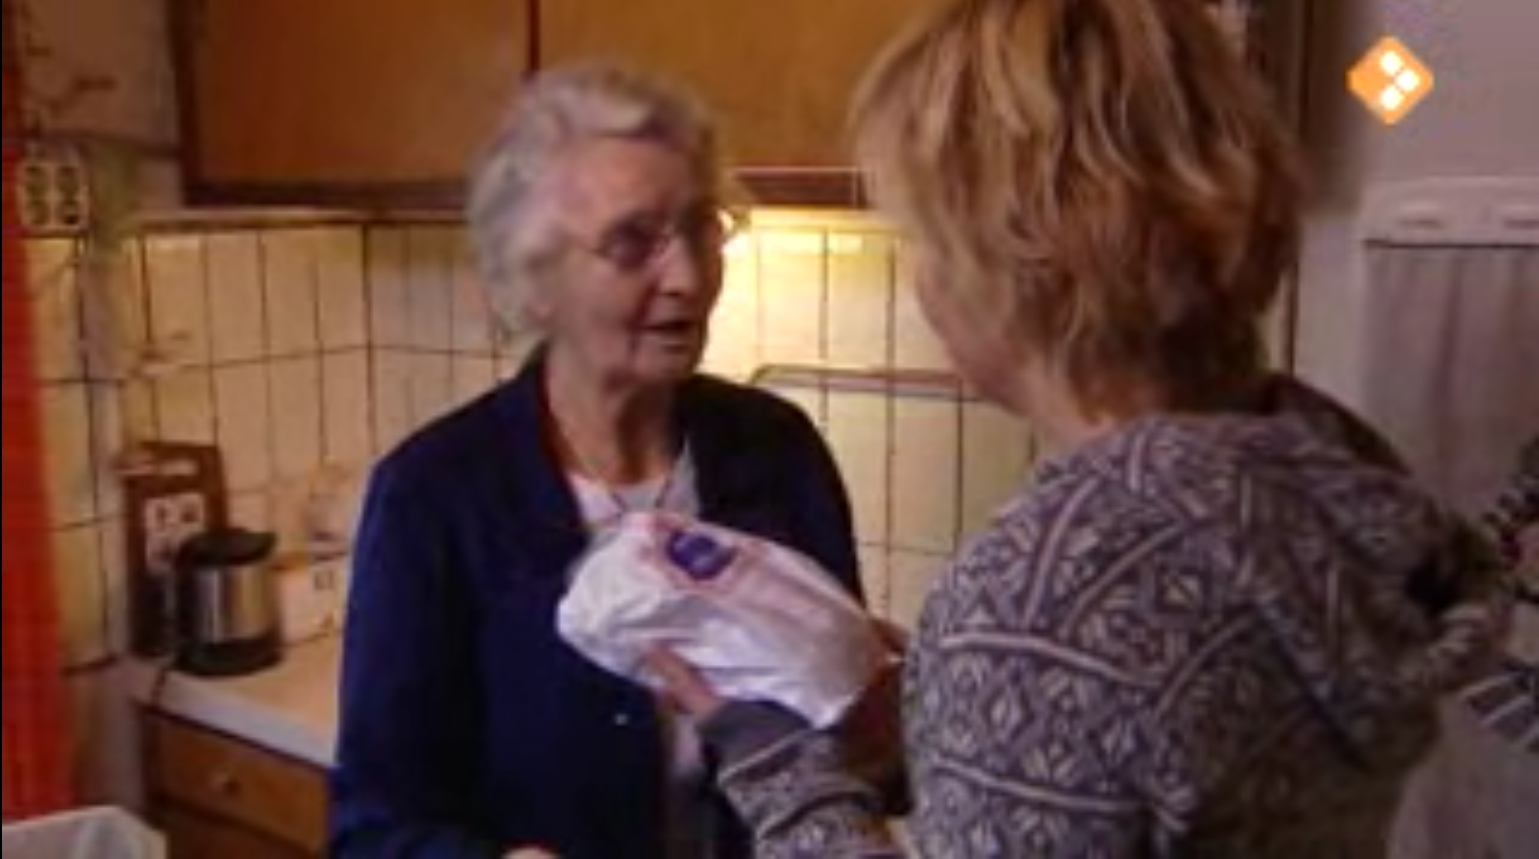
\includegraphics[scale=0.12]{kcap:bzv_screenshot} 
}
\subfigure[Example of how tags (descriptions) of the keyframe above can be classified in terms of the Panofsky-Shatford model.]{
\begin{footnotesize}
\begin{tabular*}{\columnwidth}{@{\extracolsep{\fill}}llll}
\toprule
& \textbf{Abstract} \T \B & \textbf{General} & \textbf{Specific}\\
\midrule
\textbf{Who} \T  & kind & woman &  Anna\\
             \B & lady &  &   \\
\textbf{What} & typical & present & Amsterdam\\
           \B & present &     &    sausage \\
\textbf{Where} &idyllic & kitchen& the Netherlands\\
            \B &countryside & & \\
\textbf{When} & elimination& morning &May 10th\\
	      \B & day & & 2008\\
\bottomrule	      
\end{tabular*}
\end{footnotesize}
}
\caption{Classification of user tags.}
\label{class_exmpl}
\end{figure}

\begin{table}
\begin{footnotesize}
\begin{tabular*}{\columnwidth}{@{\extracolsep{\fill}}lrrrr}
\toprule
\T \B & \textbf{Abstract} & \textbf{General} & \textbf{Specific}  \\
\midrule
\textbf{Who} \T \B & 10 & 166 &  177  & 31\%\\
\textbf{What} \B & 73 & 563 & 12 & 57\% \\
\textbf{Where} \B & 0 & 68 & 8& 7\%\\
\textbf{When} \B & 4 & 31 & 6 & 5\% \\
 \T & 7\% & 74\% & 9\% & \\
\bottomrule
\end{tabular*}
\end{footnotesize}
\label{object_tags}
\caption{Distribution of the object-level tags across the categories of the Panofsky-Shatford model.}
\end{table}


Table \ref{object_tags} shows the distribution of the object-level tags across
the categories of the Panofsky-Shatford model. Looking at the total number of
tags at the different abstraction levels, we observe that the majority of the
tags are general (74\%), while only 7\% are at the abstract level and 9\% at
the specific level. On the other hand, looking at the total number of tags in
the facets, we observe that the majority of the tags belong to the What facet
(57\%). Furthermore, a considerable number of tags are in the Who facet and
only a small number of tags belong to the Where and When facets. Looking at
the relations between the abstraction levels and the facets we observe that
almost all tags in the What facet are general, sometimes abstract, but rarely
specific. The descriptions in the Who facet are, however, at both the general
and the specific level, but rarely abstract. Most of the tags in the Where
facet are generic, and little are specific place or country names. Finally, we
encountered 195 tags that we could not classify in any of the facets. Most of
the time, these tags were modifiers --- typically adjectives and adverbs ---
that describe how an action was performed, for example nice, better etc.

Our results show similarities with classification of image annotations by
Hollink et al.~\cite{laurapaper}. They also found that a large majority of the
descriptions are at the conceptual level. She, however, found a larger number
of scenes (30\%) at the conceptual level. A possible explanation for this
difference could be the fast pace of the game, which makes the player focus on
the directly perceivable objects instead of the overall scene. The evaluation
of the tags by a professional cataloguer also suggested that the users focus
on what can be directly seen or heard. Hollink et. al also found the majority of the descriptions to be at the general level (74\%).

\section{Discussion and future work}
\label{sec:discussion}

In this section we summarize the main observations from our experiments and
discuss to what extent the tags collected with \emph{Waisda?} fulfill the aims
of the Netherlands Institute for Sound and Vision. In addition, we discuss how
the results of our study can improve future versions of the game.

From the comparison of the tags with the terms from the GTAA thesaurus of the
institute and the linguistic database of Dutch, Cornetto, we made several
observations. We can confirm that the aim of the institute to collect metadata
in a user vocabulary can be achieved with the \emph{Waisda?} video labeling game.
Comparable to the results that were found in the Steve.museum tagging project
we found small overlap with the terms in the vocabulary used by professional
cataloguers. In addition, almost half of the verified tags are valid Dutch
words, as they were found in Cornetto. 

The number of verified tags found in Cornetto is much higher than the
number of tags that are not verified. This provides evidence
for the assumption of video labeling games that user agreement on tags can be
used to filter out non-well-formed. We also observed that a large part of
the tags that are not verified could still be potentially useful. A large part
of the non-verified tags could also be found in the vocabularies. In addition,
we deemed most tags meaningful as they returned results from Google.

The manual classification of the tags provides details about the type of tags
that were collected in \emph{Waisda?} and how they relate to the video
content. Users predominately describe \emph{what} appears in the video using
generic tags. Although the tags also provide some coverage of the subject, the
\emph{who}, and the location, the \emph{when} in the video fragments. While
the persons occurring as the subject are described both in generic and
specific tags, there are very few tags describing specific locations.

Together with The Netherlands Institute for Sound and Vision we are preparing
a second pilot project with \emph{Waisda?}. The results of this study show
several limitations of the current metadata, that we aim to address in this
pilot. One limitation is the low number of specific type of tags in the
\emph{who} and \emph{where} facets. We are exploring how users can be
motivated to provide such tags. We showed that by matching the tags to
controlled vocabularies we can derive the type of the tags. We are exploring
if this can be used within the game to detect what type of tags are entered,
and for example provide more points when the user enters a location name. For
this purpose the recall of the current algorithm to match tags and terms
should be improved.

Another characteristic of the current \emph{Waisda?} tags is that many are
also found in the subtitles. In case these subtitles are also available for
retrieval this can be considered a limitation of the tags, as it reduces the
added value. Computing the overlap between the tags and the subtitles during
the game can be used to detect such tags, and for example be used to motivate
users to provide different tags.

An assumption of labeling games is that only the verified tags are associated
to the content as metadata. Our study shows that this approach would exclude
many potentially useful tags. A solution could be to include tags that can be
matched with a term from a controlled vocabulary. Another solution could be to
compare the syntactically different tags based on their semantic similarity.
We are currently exploring the consequences of these methods.

Finally, in future work we will experiment with the usefulness of the tags in
search tasks. From the current results we learned that tags describe what
users directly see or hear in the video. They do not provide a topical description
of a fragment. We expect that the current tags are, therefore, suited to find
objects within a specific video, but are as of yet less useful to find
specific fragments. In future work we will explore methods to also collect
topical descriptions of video scenes, by extending the game and/or with
post-processing of the tags after the game.
